\chapter{Introduction}
\section{Background}
An unmanned aerial vehicle (UAV) is defined as an autonomous aircraft that can fly without a human pilot on board \cite{icao16}. %"ICAO?s circular 328 AN/190 : Unmanned Aircraft Systems" (PDF). ICAO. Retrieved 3 February 2016.
A quadrotor is a UAV that consists of two pairs of counter-rotating rotors with fixed-pitch blades \cite{Hoffmann07}. %Quadrotor Helicopter Flight Dynamics and Control: Theory and Experiment?
With independent output of each motor, the quadrotor has full control of its orientation (roll, pitch, and yaw) and thrust. The quadrotor's translation motion is coupled with the quadrotor attitude and thrust since the thrust occurs in only the perpendicular direction of the quadrotor orientation; the direction of the translation is determined by the orientation, and the magnitude of the translation is determined by the thrust. Therefore, the quadrotor controls its translation by altering its attitude and has a capacity of both rotation and translation maneuvers. Due to the advantage, quadrotors have been used for various purposes and performed tasks in environments that are nearly impossible to reach as a human. As an example, Michael et al. developed an autonomous quadrotor to explore an earthquake-damaged building with multiple floors collaborating with a ground robot \cite{Michael02}. %Collaborative Mapping of an Earthquake-Damaged Building via Ground and Aerial Robots
Chambers et al. developed a quadrotor system that maps rivers with a self-supervised river classification system \cite{Chambers11}.
%Perception for a River Mapping Robot

A control system for quadrotors usually consists of position control (outer-loop) and attitude control (inner-loop). Position control maps input of translation motion into desired orientation and thrust. Attitude control computes desired torque corresponding to the desired and current attitude. However, because of factors like rotational effects on translation motion, and aerodynamic effects, the dynamic model of the quadrotor is highly non-linear. Therefore, there is a demand of advanced control system for the quadrotor's performance.

\section{Related Works}
For improvement of quadrotors' performance, various research on advanced control systems for a quadrotor have been conducted actively. Raffo et al. applied a nonlinear \({\mathscr{H}}_{\infty}\) control to attitude control and designed a backstepping control for path tracking of a quadrotor. The control system was evaluated by simulations \cite{Raffo08}. %Backstepping/Nonlinear H? Control for Path Tracking of a QuadRotor Unmanned Aerial Vehicle
Morgan et al. designed and implemented a dynamic-model-based nonlinear attitude control in the swarm assignment and trajectory optimization \cite{Morgan16}. %Swarm assignment and trajectory optimization using variable-swarm, distributed auction assignment and sequential convex programming
In the case of the application of adaptive control, Mallikarjunan et al. demonstrated an application of \({\mathscr{L}}_{1}\)  adaptive control for quadrotors' attitude control by experiments \cite{Mallikarjunan12}. %L1 Adaptive Controller for Attitude Control of Multirotors
Also, Diao et al. suggested a Lyapunov based nonlinear adaptive control for a quadrotor under uncertainties of mass, inertia, and aerodynamic damping coefficients, and evaluated the control by simulations \cite{Diao11}. %A Nonlinear Adaptive Control Approach for Quadrotor UAVs

On the other side, trajectories of a quadrotor is also studied by many researchers to improve its performance. 
Ritz et al. designed a method to compute a quardrotor's time-optimal trajectory between two given states, and evaluated the method by simulations \cite{Ritz11}.
%Quadrocopter Performance Benchmarking Using Optimal Control
Mellinger et al. developed an algorithm of a trajectory generator for a quadrotor's aggressive maneuvers, and validated the quadrotor's performance by experiments \cite{Mellinger12}.
% Trajectory generation and control for precise aggressive maneuvers with quadrotors
In addition, Dierksand and Jagannathan suggested a control scheme that uses control inputs computed by neural networks \cite{Dierks10}. %Output Feedback Control of a Quadrotor UAV Using Neural Networks

Here, we develop a model based attitude control system focused on addressing the nonlinearity of quadrotor dynamics in order to improve agility and stability.

\section{Motivation}

Due to high nonlinearities of quadrotor dynamics, application of advanced controllers is expected to improve performance of the quadrotor, compared with conventional controllers, such as PID and Linear-Quadratic Regulator. Studies of quadrotor dynamics are expected to increase the robustness of the control systems.

The Aerospace Robotics and Control Laboratory at the University of Illinois had developed quadrotor platforms based on Crazyflie 1.0 to validate performance of nonlinear controllers \cite{Morgan16}.  %Swarm assignment and trajectory optimization using variable-swarm, distributed auction assignment and sequential convex programming
Crazyflie is a open-source nano quadrotor system developed by Bitcraze \cite{bitcraze}. %https://www.bitcraze.io
A Crazyflie quadrotor is about 19 g weight and each leg is about 6 cm length. However, due to the quadrotor's physical constrains, such as its load limit and sensor errors, its application is limited. Especially, in order to develop a vision-based position control system and other high-level functions for the quadrotor, only 8 g of load is allowed for sensors, equipments, and mount for them, and therefore, choice of sensors and algorithms is limited. A Crazyflie quadcopter with a camera and mount is shown in Figure \ref{fig:crazyflie}.

\begin{figure}
    \centering
    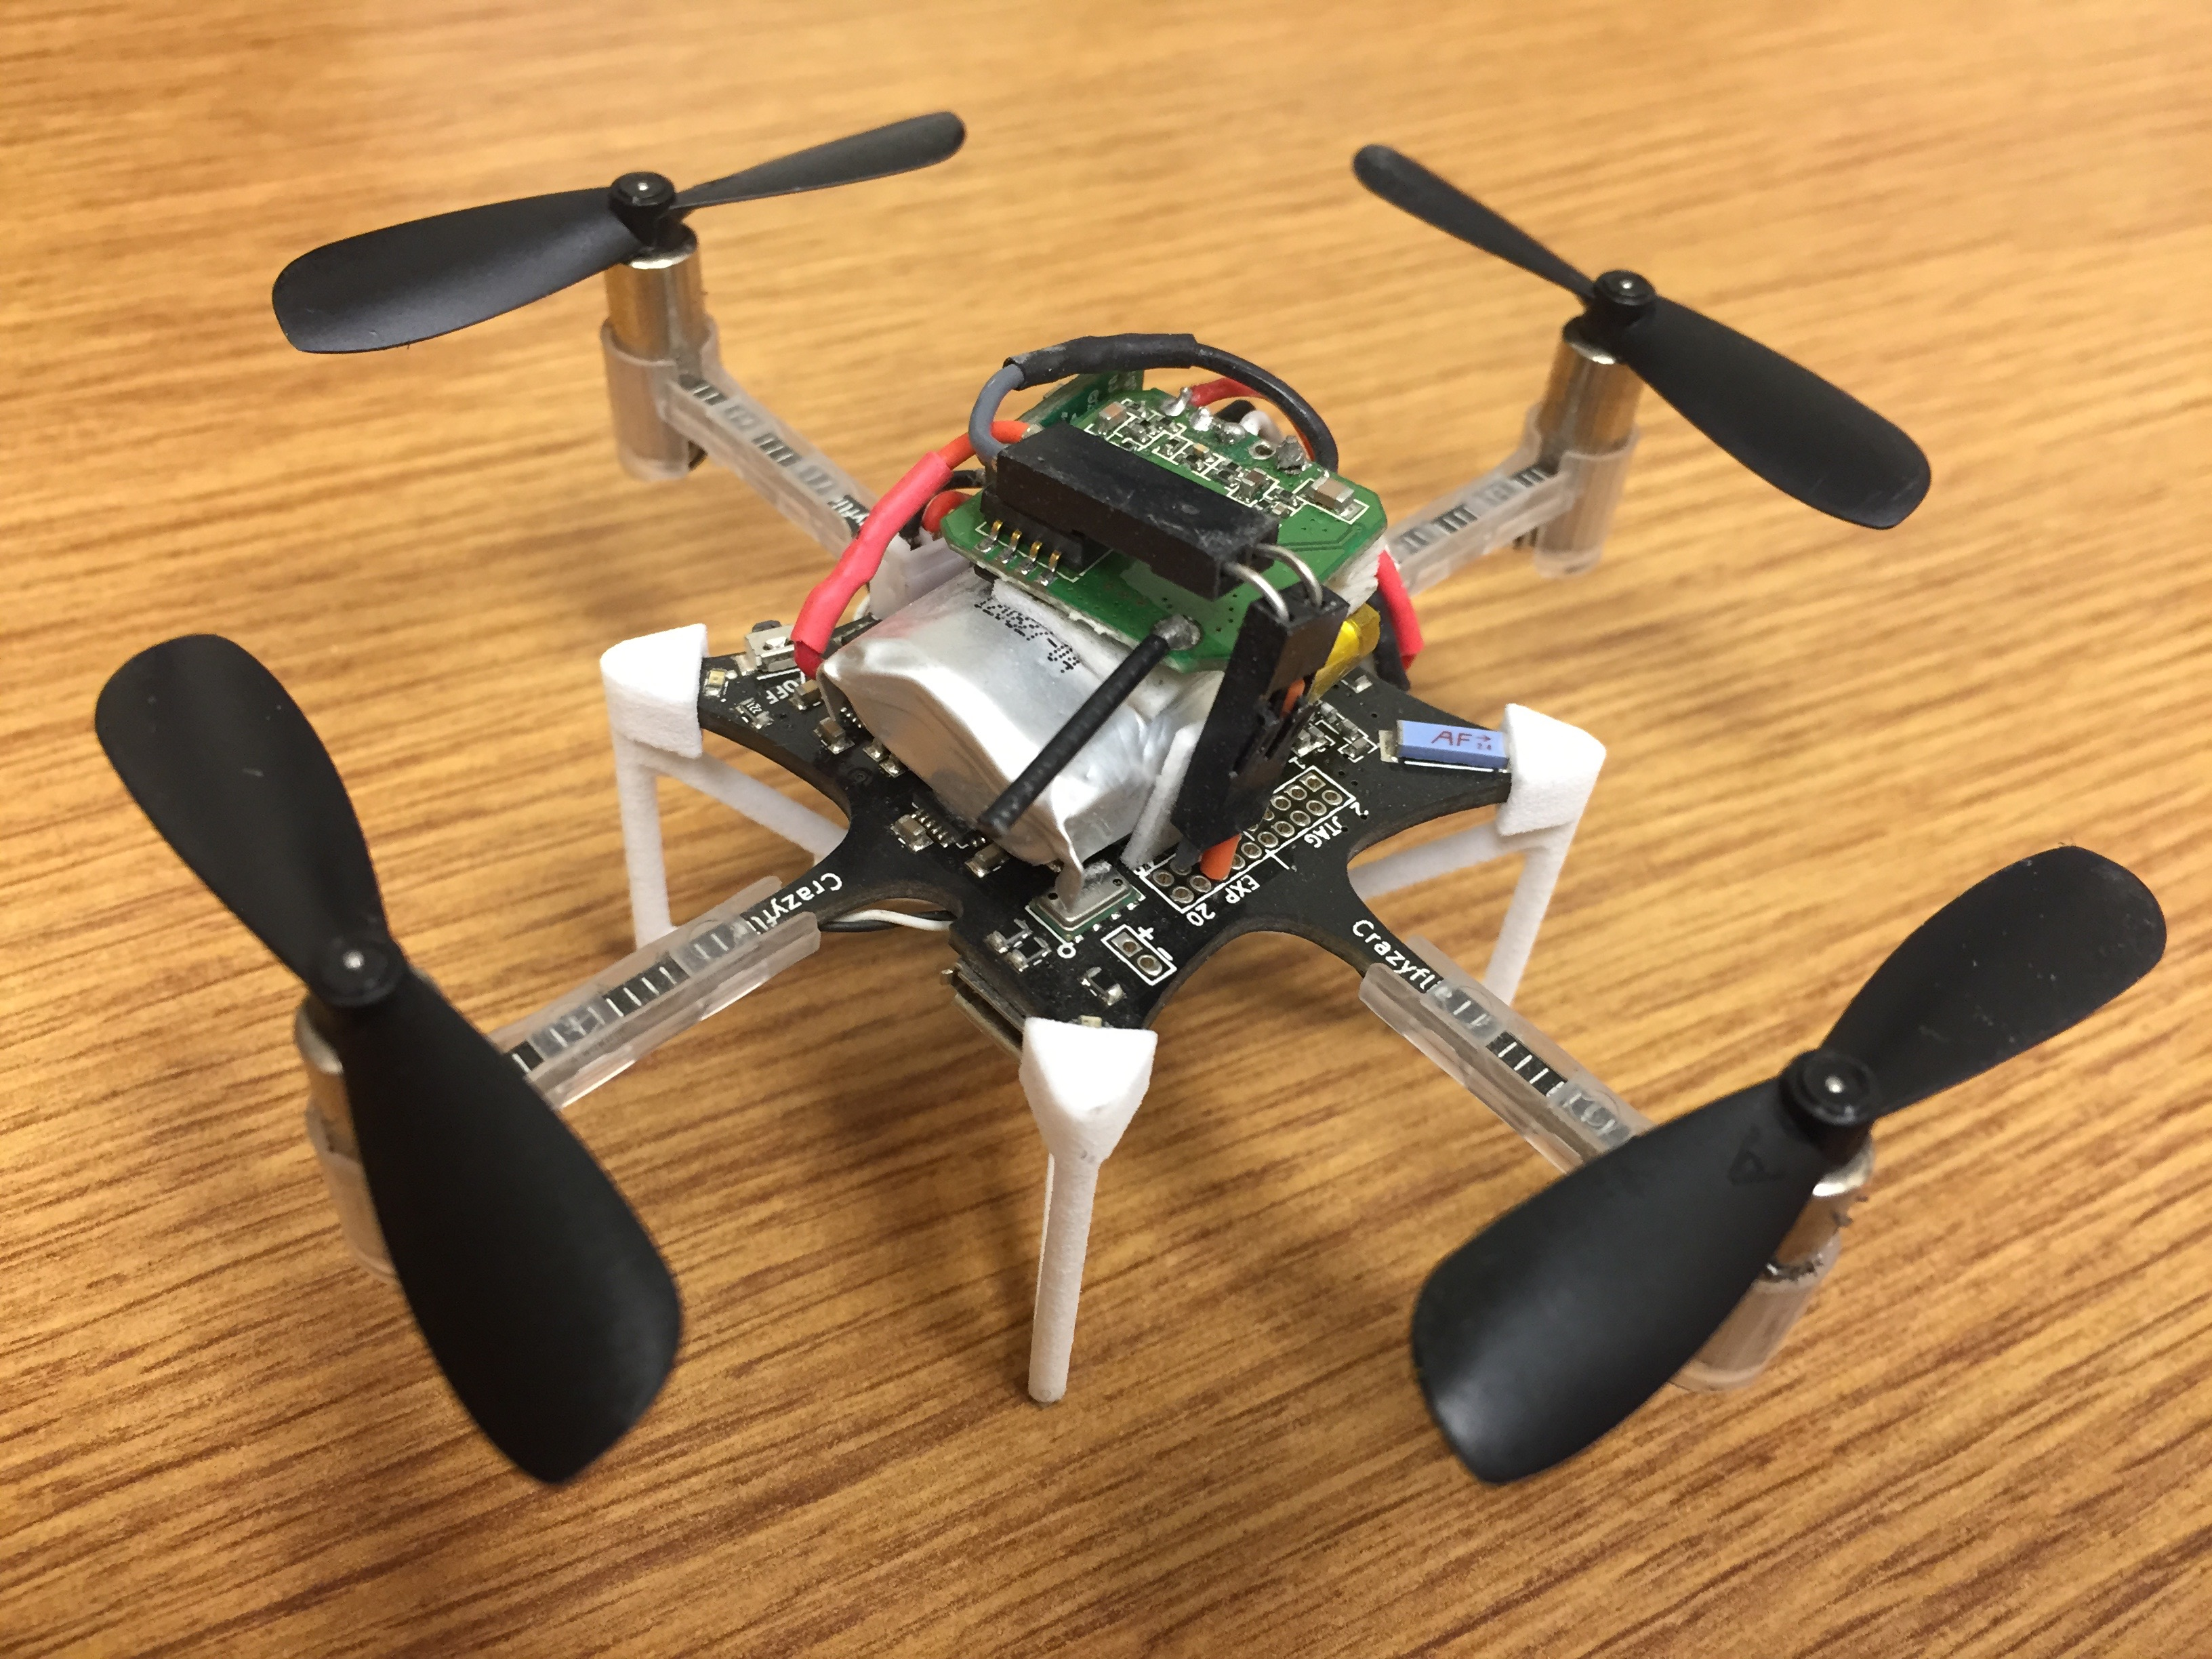
\includegraphics[width=0.5\textwidth]{graphics/crazyflie.jpg}
    \caption{A Crazyflie Nano Quadrotor with a Downward Camera}
    \label{fig:crazyflie}
\end{figure}

In order to solve such problems, a micro quadrotor can be used alternatively. With greater load capacity, a micro quadrotor can equip with various light-weighted devices onboard, such as a wide-angle camera and a companion computer. In addition, more various autopilot systems are available for a micro quadrotor than for a nano quadrotor. For these advantages, a micro quadrotor is expected to be a better research platform for various purposes, and therefore, this research aims for developing a new micro quadrotor system.

\section{Objective}

In this research, we aim for the application and evaluation of the nonlinear attitude control, suggested by Bandyopadhyay and Chung, that was originally designed for a spacecraft \cite{Bandyopadhyay16}. %Nonlinear Attitude Control of Spacecraft with a Large Captured Object
Also, we validate the proposed approach of inner-loop nonlinear attitude control and linear outer-loop position control with feedforward cancellation used in \cite{Morgan16}. In order to implement the control system, we developed a new micro quadrotor system. The quadrotor dynamics is modeled and characterized based on experimental data. Performance of the quadrotor with the nonlinear attitude control is evaluated by both flight experiments and simulations and compared with conventional PID attitude control. In addition, we suggest a computationally-efficient algorithm to estimate the position of the quadrotor by capturing image data of visual markers, and the algorithm is evaluated by experiments, independently from the quadrotor's flight.

\section{Outline}

The thesis is organized as follows. Chapter \ref{ch:system} describes the overview of the quadrotor system. Chapter \ref{ch:system} also describes the hardware specification of each component and the physical properties of the quadrotor. Chapter \ref{ch:control_system} focuses on the dynamic model and the control system. To be more specific, Section \ref{sec:control_system_system_overview} presents the control system overview. Section \ref{sec:coordinate_system} defines the coordinate systems used for the quadrotor system. Section \ref{sec:outer_loop} describes the dynamic model of the quadrotor's translation motion and its position control. Section \ref{sec:inner_loop} presents the dynamics of the quadrotor rotation and the nonlinear attitude control. The proof of the stability of the nonlinear control is also stated in this section. In Section \ref{sec:motor_control}, a model of DC motors is introduced and an open-loop control of the motors is described. Chapter \ref{ch:evaluation} presents the evaluation of the control system that is stated in Chapter \ref{ch:control_system}. In particular, Section \ref{sec:pid} describes an PID attitude control that is compared with the nonlinear control system. Section \ref{sec:simulation} discusses numerical simulation results of the nonlinear and PID attitude control of the quadrotor. In Section \ref{sec:experiment}, the results of flight experiments are presented with various inputs. Chapter \ref{ch:vision_based_control} introduces a computationally-efficient method to estimate the quadrotor position with given image data of visual markers, and discusses performance of the algorithm. Finally, Chapter \ref{ch:conclusion} summarizes the contents of this thesis and suggests future works.